\documentclass[11pt,a4paper]{article}

\usepackage[brazil]{babel}
\usepackage[utf8]{inputenc}
\usepackage[T1]{fontenc}
\usepackage{graphicx}
\usepackage{float}

\floatstyle{boxed}
\restylefloat{figure}
\author{Carlos Eduardo Elmadjian, Ricardo Mikio Morita e Gil Santaella}
\author{
  Elmadjian, Carlos Eduardo\\
  \texttt{elmadjian@linux.ime.usp.br}
  \and
  Morita, Ricardo Mikio\\
  \texttt{ricardom@linux.ime.usp.br}
  \and
  Santaella, Gil\\
  \texttt{gssantaella@gmail.com}
}
\linespread{1}
\setlength{\parindent}{0.5cm} 

\title{Guia do Usuário: Canoagem}
\begin{document}
\maketitle

\section*{Introdução}
\thispagestyle{empty}
\vspace{1cm}
\begin{center}
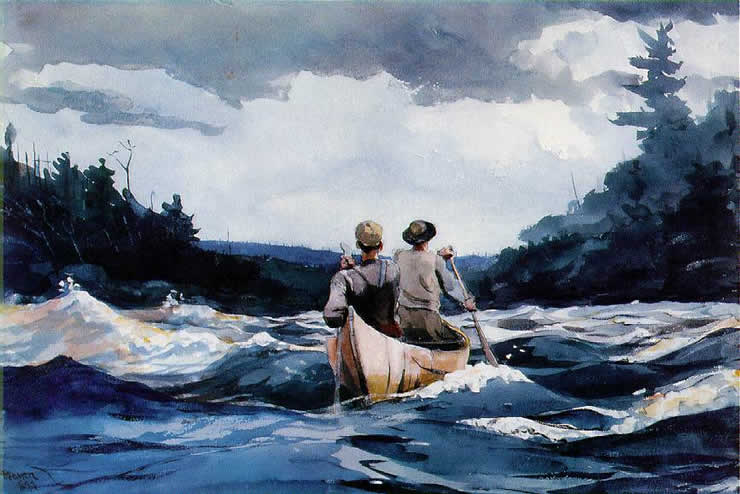
\includegraphics[scale=3.5]{CanoeInTheRapids.jpg}
\end{center}
\vspace{1cm}
\begin{flushright}
{\footnotesize \textit{"Cada um rema sozinho uma canoa que navega um rio diferente\\
 mesmo parecendo que esta pertinho."}\\ \textbf{Guimarães Rosa}}
\end{flushright}

Este documento tem como papel descrever o funcionamento do executável de Canoagem para o usuário. Nas seções a seguir, descreveremos a forma de se usar o programa.

\section{Compilação}
\setcounter{page}{1}

Para compilar o programa, simplesmente rode no seu shell preferido:\\

\verb|> make| \\

O programa \textit{make} irá gerar um executável com o nome \textit{main}.
	
\section{Execução}
Para executar o programa main digite no seu shell preferido:\\

\verb|>./main| \\

Isso fará com que o programa exiba o seguinte menu:
\begin{center}
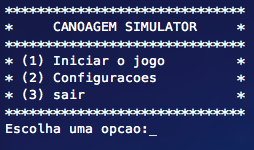
\includegraphics[scale=0.6]{menu.png}
\end{center}

O programa irá carregar por padrão um arquivo de configurações iniciais com o nome de \verb|config.txt|. Nesse arquivo, estão dispostas 16 opções, entre elas algumas exclusivas para modo depuração, que definem como o jogo deverá se comportar.\\

Para aceitar este arquivo e iniciar o jogo, digite 1 na tela inicial.\\

Se desejar, o usuário poderá visualizar ou ainda alterar essas configurações. Para isso, digite 2 na tela inicial. Essa opção irá mostrar um menu de configurações como abaixo (para saber mais sobre cada opção, por favor, confira o arquivo \verb|./debug/config.txt|):\\
\begin{center}
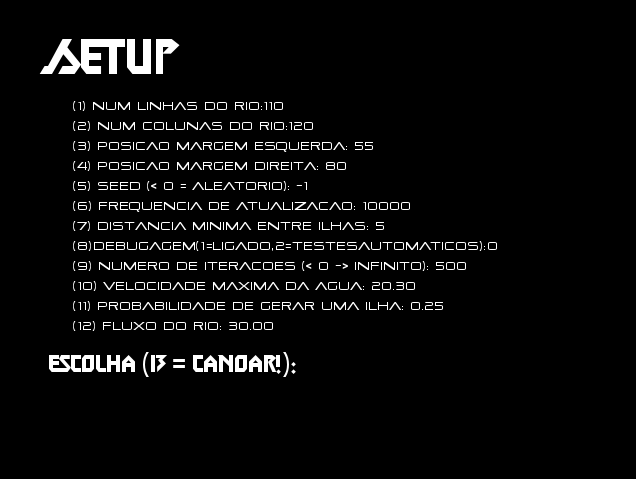
\includegraphics[scale=0.6]{config.png}
\end{center}
\vspace{0.5cm}
Ainda é possível adicionar entradas que sobrescreverão as do arquivo de configuração. Para isto, basta \textit{adicionar à chamada do executável os parâmetros desejados}. Segue abaixo uma tabela com as opções disponíveis: \\
\begin{center}

\begin{tabular}{|c|c|c|}
\hline 
Argumento & Variável & Exemplos de uso \\ 
\hline 
-nl & Número de linhas & -nl10, -nl100, -nl1000 \\ 
\hline 
-nc & Número de colunas & -nc20, -nc50, -nc80 \\ 
\hline 
-lm & Limite esquerdo do rio & -lm5, -lm30, -lm100 \\ 
\hline 
-rm & Limite direito do rio & -rm10, -rm50, -rm200 \\ 
\hline 
-rr & Refresh Rate(microsegundos) & -rr10000, -rr5000, -rr12000 \\ 
\hline 
-id & dist.mínima entre ilhas & -id5, -id2, -id8 \\ 
\hline 
-fl & Fluxo de água do rio & -fl50, -fl20, -fl35 \\ 
\hline 
-ig & Prob. de gerar ilhas & -ig0.5, -ig0.2, -ig0.9 \\ 
\hline 
-it & Número de iterações & -it20, -it100, -it0 \\ 
\hline 
-rd & 1:relatório, 2:teste de robustez & -rd0, -rd1, -rd2 \\ 
\hline 
-ie & Ignora erros (para debug) & -ie0, -ie1 \\ 
\hline 
\end{tabular} 
\end{center}

Se você estiver bastante arrependido, você ainda pode sair do programa digitando 3 no menu inicial. De toda forma, ao final do jogo, o programa terminará sua execução.

\section{Gameplay/Como Jogar}
A canoa deve ser controlada com as setas esquerda e direita do teclado. Para ganhar mais velocidade, o usuário deve remar mais, isto é, fazer a canoa ir de um lado para o outro. Quanto mais rápido a canoa se move, mais pontos o usuário conquista.

A velocidade exibida na tela corresponde à velocidade da canoa relativa à água. Portanto, o jogador não ganha pontos se não remar, embora a canoa possa estar se movimentando em função da velocidade do rio.

Em cada partida, o jogador sempre começa com três vidas (representadas por corações vermelhos). Há uma barra de \textit{“health points” (HP)} que indica qual o nível de cada coração. Quando perde uma vida, um dos corações do jogador se apaga. 

Sempre que há colisões entre a canoa e ilhas ou margens, a barra de HP do jogador é gradualmente reduzida. É muito importante que o usuário tente se livrar de um objeto com o qual se chocou o mais rápido possível para que sua barra de HP não diminua ainda mais.

\begin{center}
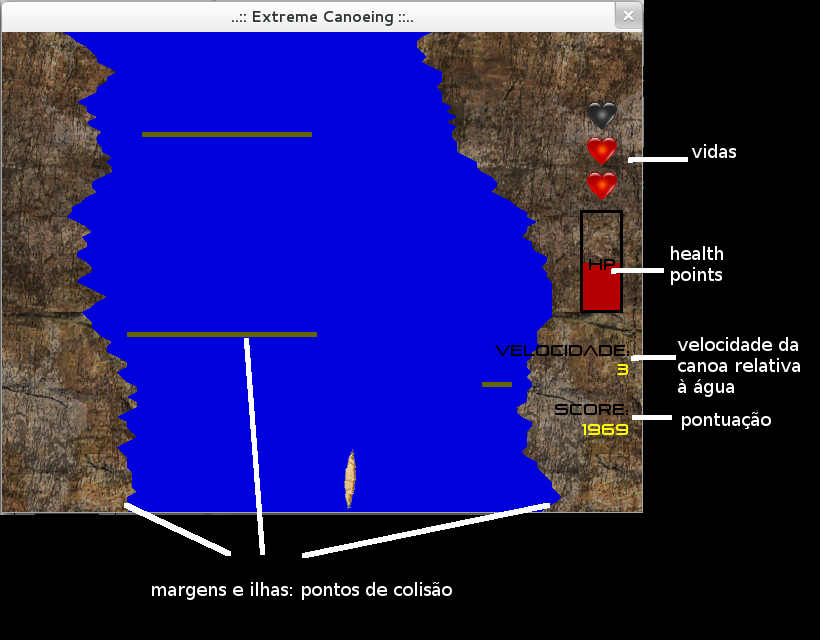
\includegraphics[scale=0.4]{explicacao.jpg}
\end{center}

Ao longo do jogo, o usuário também poderá perceber que a correnteza do rio vai aumentando em função do número de pontos que ele conquista. Quando isso acontece, a navegação se torna mais rápida e a canoa fica mais difícil de controlar.

\begin{center}
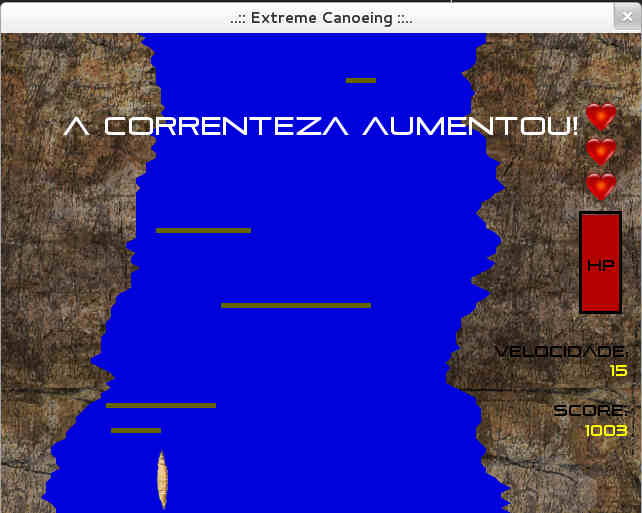
\includegraphics[scale=0.5]{correnteza.jpg}
\end{center}

Ao perder os três corações, o jogo termina e a tela exibe a pontuação que o jogador conquistou naquela partida.

\begin{center}
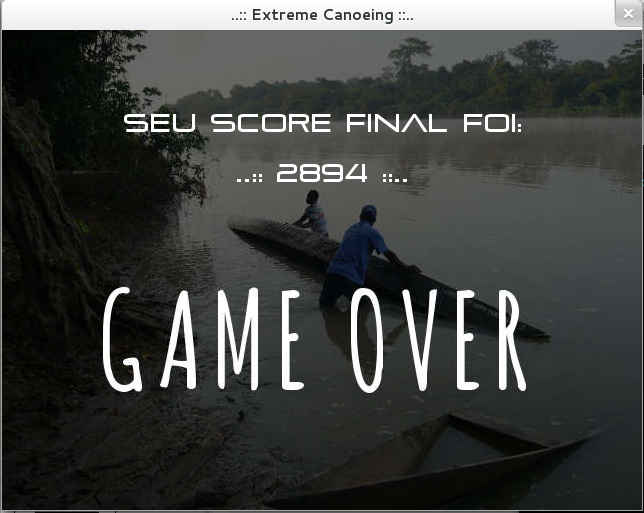
\includegraphics[scale=0.5]{gameover.jpg}
\end{center}

\section{modo depuração}
Para executar o programa main no modo depuração, você deve alterar a opção 8 do menu de configurações para o valor 2 (ou usando \verb|./main -rd2|). Isso fará com que o programa realize uma série de testes de robustez, correção e variações sobre o rio que é gerado. Nos testes de robustez, serão carregados arquivos pré-configurados com condições extremas. Até por isso, é natural não esperar correção de valores de fluxo, por exemplo, pois queremos apenas que o programa sobreviva. \\

Se para a opção 8, modo de debugagem, você digitar 1, o programa fará um teste com as opções carregadas no menu e mostrará algumas informações sobre o programa. 

\end{document}